\documentclass[11pt,a4paper,boxed]{caspset}

% set 1-inch margins in the document
\usepackage[left=1in,right=1in,top=1.2in,bottom=1in]{geometry}
\usepackage{amsmath,amsfonts,amsthm,amssymb}
\usepackage{hyperref}
\usepackage{setspace}
\usepackage{lastpage}
\usepackage{chngpage}
\usepackage{soul}
\usepackage[usenames,dvipsnames]{color}
\usepackage{graphicx,float,wrapfig}
\usepackage{ifthen}
\usepackage{listings}
\usepackage{courier}
\usepackage{multimedia}
\usepackage{color, soul}
\usepackage{indentfirst}
\usepackage{wrapfig}
\usepackage{picinpar}
\usepackage{xypic}
\usepackage{fancyhdr}

%%%%%%%%%%%%%%%%%%%%%%%%%%%%%%%%%%%%%%%%%%%%%%%%%%%%%%
\usepackage{xeCJK}
%\usepackage{fontspec}
\setCJKmainfont[BoldFont=simhei.ttf]{simsun.ttf}
%\setCJKsansfont{simhei.ttf}
%\setCJKmonofont{simfang.ttf}

%\setCJKmainfont{Adobe Song Std}
%\setCJKmainfont[BoldFont=Adobe Heiti Std]{Adobe Song Std}
%%%%%%%%%%%%%%%%%%%%%%%%%%%%%%%%%%%%%%%%%%%%%%%%%%%%%%

\newlength\picwidth
\setlength\picwidth{0.23\textwidth}
\newlength\pichigh
\setlength\pichigh{1.277\picwidth}
%\graphicspath{{figures/}}
% Homework Specific Information
\renewcommand\refname{\bf 参考文献}
\renewcommand\contentsname{\bf 目 \ \ \ 录}
\renewcommand\figurename{\bf 图}
\renewcommand\tablename{\bf 表}

%\newtheorem{dingyi}{\bf 定义~}[section]
%\newtheorem{dingli}{\bf 定理~}[section]
%\newtheorem{yinli}[dingli]{\bf 引理~}
%\newtheorem{tuilun}[dingli]{\bf 推论~}
%\newtheorem{mingti}[dingli]{\bf 命题~}


\newcommand{\hmwkTitle}{近现代科学技术史}
\newcommand{\hmwkSubTitle}{近现代科学技术史} % No subtitle, so this will be excluded
\newcommand{\hmwkDueDate}{\today}
\newcommand{\hmwkClass}{物理学院}
\newcommand{\hmwkClassTime}{Tue./Thu.{~}13:30}
\newcommand{\hmwkClassInstructor}{刘红}
\newcommand{\hmwkAuthorName}{周吕文}

\hypersetup{pdfauthor={\hmwkAuthorName}, 
            pdftitle={近现代科学技术史}, 
            pdfsubject={\hmwkTitle, \hmwkClassInstructor},
            pdfkeywords={近现代科学技术史},
            pdfproducer={XeLateX with hyperref},
            pdfcreator={Xelatex}}

%% Setup the header and footer
\pagestyle{fancy}                                                       %
\lhead{\hmwkAuthorName}                                                 %
\chead{\hmwkClass\ (\hmwkClassInstructor): \hmwkTitle}  %
\rhead{第\ \thepage\ 页,{~} 共\ \protect\pageref{LastPage} 页}          %                                %
\definecolor{DarkGreen}{rgb}{0.0,0.45,0.0}

%%%%%%%%%%%%%%%%%%%%%%%%%%%%%%%%%%%%%%%%%%%%%%%%%%%%%%%%%%%%%

\setlength{\parskip}{5pt}
%%%%%%%%%%%%%%%%%%%%%%%%%%%%%%%%%%%%%%%%%%%%%%%%%%%%%%%%%%%%%

% info for header block in upper right hand corner
\name{周吕文{~}201128000718065}
\class{物理学院{~}20110308班}
\assignment{期末作业}
\duedate{11/24/2011}

\begin{document}

\problemlist{\LARGE 数学是科学的女王}

\section{引言}

数学家高斯曾说过: ``Mathematics is the queen of the sciences''(数学是科学的女王). 在此, 我引用高斯的话作为本文的标题, 以说明数学之于科学发展的重要地位.

至于本文为何选这个题, 源于我在听刘红老师讲孟德尔之所以能够发现遗传规律, 是由于他将数学的分析手段与方法引入了生物学. 实际上, 回顾整个科学史, 我们很容易发现, 数学是一切自然科学的基础. 正如伽里略所说, 自然界这部伟大的书是用数学语言写成的. 物理学, 力学, 天文学, 化学, 生物学, 心理学等许多科学学科的每一次重大的突破, 无一例外的依赖于数学. 天才中又岂只是孟德尔成于数学? 开普勒, 伽里略, 牛顿, 麦克斯维, 爱因斯坦等一系列科学巨匠也无一例外的同时是数学家或者数学造诣很深.

\section{天才与数学}
科学史上能说明数学在自然科学发展中起到巨大作用的例子很多, 本文从几个重要的科学学科, 列举部分科学天才是如何利用数学取得巨大成就的, 以此证明``数学在自然科学发展起了巨大作用''的这个显而易见的观点, 并作相应的评论.
\subsection{开普勒与开普勒定律}

开普勒行星运动三定律的发现为经典天文学奠定了基石, 促成了数十年后万有引力定律的发现. 可以说开普勒行星运动三定律是始于第谷, 而成于开普勒. 这与开普勒在数学方面具有的极高的才华是分不开的. 下面介绍一下开普勒的生平以及发现开普勒定律的过程.

\begin{window}[0,0,{\mbox{%
\fbox{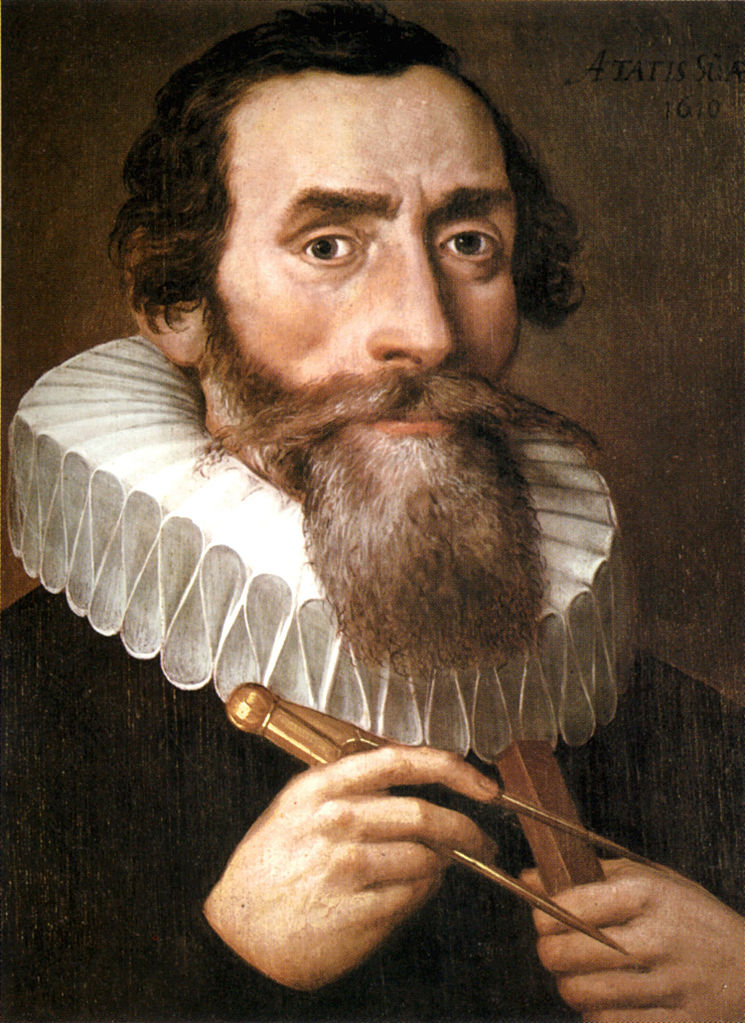
\includegraphics[width=\picwidth,totalheight=\pichigh]{./figures/kepler.jpg}}}},{}]
开普勒于1571年12月27日早产于德国威尔的一个贫民家庭, 体质很差, 四岁时患上了天花和猩红热, 受到了严重的摧残.

开普勒于1587年在蒂宾根大学读书, 受到迈克尔$\cdot$马斯特林的影响而信奉哥白尼的日心说. 毕业后, 受聘担任格拉茨的新教神学院教师. 其后, 开普勒离开格拉茨前往布拉格, 替第谷$\cdot$布拉赫从事天文观测. 1601年第谷逝世前将自己所有的天文观测资料赠给开普勒. 1627年开普勒的$\ll$鲁道夫星行表$\gg$问世.
1596年, 开普勒在宇宙论方面的著作$\ll$宇宙的奧秘$\gg$出版. 1609年开普勒发表了关于行星运动的两条定律, 1618年发现了第三条定律, 就是后来的``开普勒定律''.
1630年11月, 开普勒在雷根斯堡病逝.
\end{window}

第谷认为, 如果哥白尼的日心学说是对的, 那么必然能在不同的季节, 观测到恒星间相对位置的发生变化. 但受到当时观测条件限制, 根本无法观测到如此微小的差异. 第谷观测了一生也没有发现视差. 但第谷的观测是极为仔细的, 他留下了大量的观测资料, 并把这些珍贵的资料遗留给了开普勒.

鲁道夫皇帝资助使得第谷观测整理了大量的恒星数据, 然后由开普勒这样具有高超的数学技巧天才使用. 使得新的宇宙观注定最后在布拉格产生: 一个宇宙模型把太阳作为中心而不是地球.
显然这已经不是什么新观点, 早在古希腊, 印度和阿拉伯的天文学家就讨论过了,
后来又被哥白尼重新发现, 但其观点至死也不被人接受. 多年后的开普勒确信哥白尼的日心学说, 并认为太阳拥有某种力量以驱动行星绕其运行,
因此, 运用第谷留下的数据, 他给了自己一个几乎无法完成的挑战: 解释运动最为奇怪的火星的运行. 他相信他能通过地球和火星绕日运动的轨道
来解释这种运动. 有了泰科数据的支撑, 他开始用数学方法去证明. 这是难以想像的乏味而冗长的工作, 成百上千页的计算花了他5年多的时间. 没有极高的数学才华是完成不了的.
以至他后来写到``亲爱的读者,
如果你对这些计算感到厌倦, 那么请想想我已经做了70次了''. 开普勒尝试所能想到的各种方式, 改变行星速度, 转换轨道... 但是不管怎么做, 圆形轨道都无法与泰科精确的观测数据相匹配. 于是他做了十分大胆的假设, 以椭圆轨道替代了之前的圆形轨道, 最后他终于创造出了匹配观测证据的宇宙模型.

开普勒摧毁了一座由托勒密修建的屹立了2000年的大型建筑, 取而代之是他的第一套行星运转规则(开普勒定律):
\begin{itemize}
\item \textbf{轨道定律}: 每一个行星都沿各自的椭圆轨道环绕太阳, 而太阳则处在椭圆的一个焦点中.
\item \textbf{面积定律}: 在相等时间内, 太阳和运动着的行星的连线所扫过的面积都是相等的.
    \[
    \frac{dS}{dt}=\frac{r\cdot (v dt)/2}{dt} = \mathrm{constant} \Longrightarrow  \mathbf{v}\cdot \mathbf{r} = \mathrm{constant}
    \]
\item \textbf{周期定律}: 各个行星绕太阳公转周期($\tau$)的平方和它们的椭圆轨道的半长轴($a$)的立方成正比(比例系数为$K$).
    \[
    \frac{a^3}{\tau^2} = K
    \]
\end{itemize}
\begin{figure}
\centering
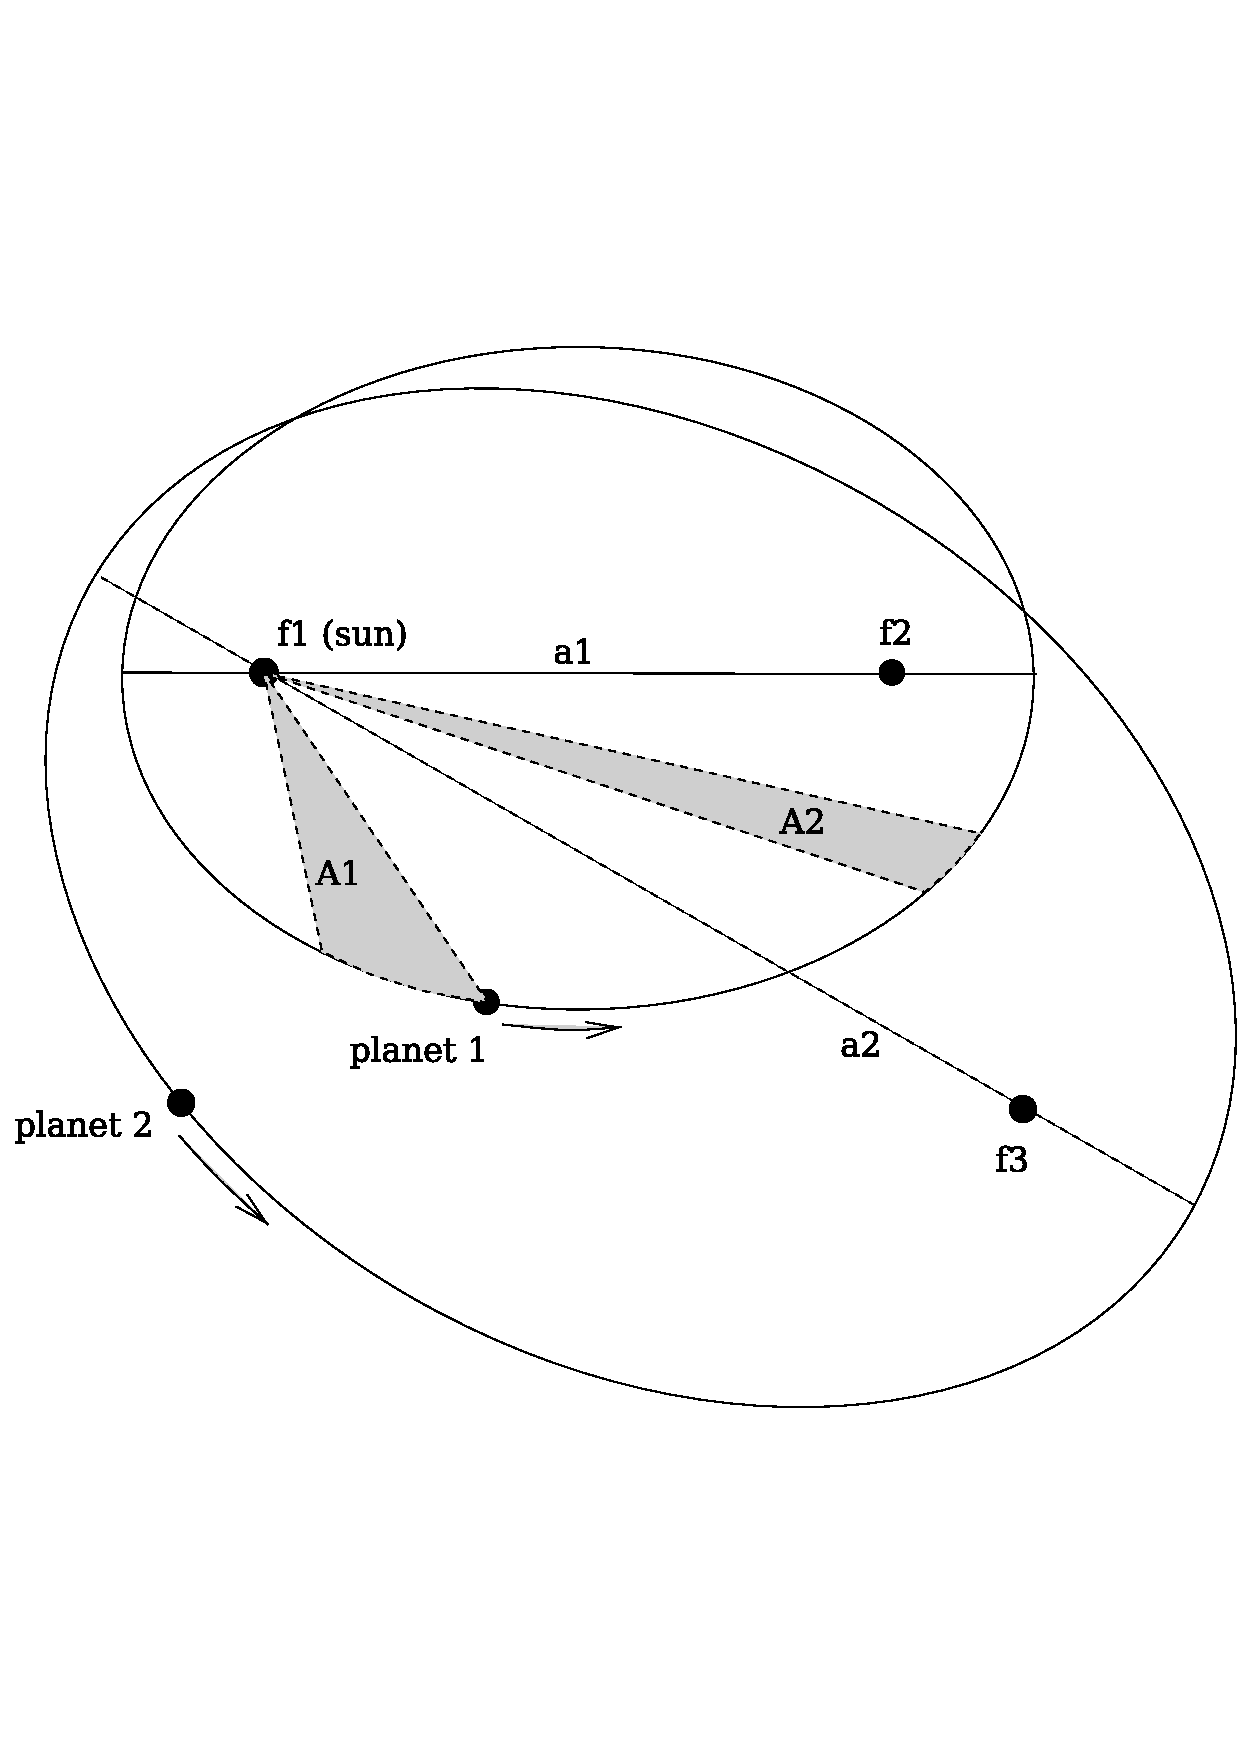
\includegraphics[width=0.4\textwidth]{./figures/keplerLaws.pdf}
\caption{\label{keplerLaws}开普勒定律}
\end{figure}

从开普勒发现开普勒定律的过程中, 我们可以发现, 没有高超的数学技巧(包括代数运算和几何分析), 开普勒也只能和第谷一样, 测些看不懂的数据罢了. 只有当精确测量的数据遇到具有极高数学细胞的大脑, 真理才能被人类所发现. 第谷算幸运的, 他的数据遇到开普勒这样伟大的数学能手, 否则他的数据将沉睡百年或者更久. 开普勒的这个例子告诉我们, \textbf{突破性的科学发现{}= 精确的数据 + 高超的数学}.

\subsection{牛顿与万有引力定律}
万有引力定律是物理, 力学以及天文学是一个重大的发现. 万有引力和牛顿三大运动定律, 奠定了此后三个世纪里物理世界的科学观点, 并成为了现代工程学的基础.
而牛顿之所以能发现万有引力定律, 其高明的地方就在于他解决了胡克等人没有能够解决的数学论证问题. 下面介绍一下牛顿的生平以及发现万有引力定律的过程.
\begin{window}[0,0,{\mbox{%
\fbox{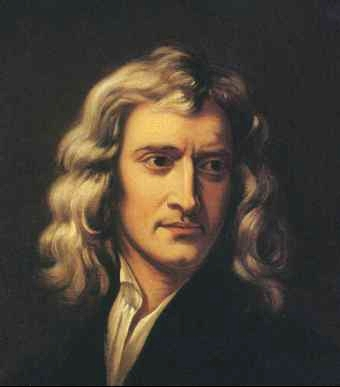
\includegraphics[width=\picwidth,totalheight=\pichigh]{./figures/Newton.jpg}}}},{}]
1643年1月4日, 艾萨克$\cdot$ 牛顿出生于英格兰林肯郡乡下的落埃尔斯索普村的埃尔斯索普庄园.
牛顿出生前, 其父亲刚去世, 牛顿3岁时, 其母改嫁. 从12岁左右到17岁, 牛顿在国王中学学习. 1661年6月, 进入了剑桥大学. 1665年, 他发现了广义二项式定理, 在1665年, 牛顿获得了学位.在此后两年里, 牛顿在家中继续研究微积分学,光学和万有引力定律.
1667年3月, 牛顿返回剑桥大学, 同年10月,牛顿被任命为剑桥大学卢卡西讲座的数学教授.
1684年牛顿开始撰写他的$\ll$自然哲学的数学原理$\gg$并于1687年出版.
1703年11月30日,牛顿被选为皇家学会主席.
1704年牛顿有关光的研究的著作$\ll$光学$\gg$出版.
1727年 3月30日, 牛顿爵士逝世, 享年84岁.
\end{window}

实际上在牛顿发现万有引力定律之前, 就有一些科学家几乎就要发现引力定律.
 比如此前开普勒就认识到要维持行星沿椭圆轨道运动必定有一种类似磁力的力在起作用.
 1659年, 惠更斯研究摆的运动时发现保持物体圆周运动需要一种向心力并于1673年, 推导出向心力定律.
1664年, 胡克发现彗星靠近太阳时轨道弯曲是由于太阳对彗星有引力作用的结果; 1679年, 胡克和哈雷根据向心力定律和开普勒第三定律, 推导出维持行星运动的向心力和距离的平方成反比. 即
\[
F = \frac{K}{r^2}
\]
显然这已经非常接近万有引力定律的最终形式.

1679年, 胡克曾写信问牛顿, 能不能由向心力定律和引力同距离的平方成反比的定律, 来证明行星沿椭圆轨道运动. 牛顿没有回答这个问题. 1685年, 哈雷登门拜访牛顿时, 牛顿已经发现了万有引力定律: 两个物体之间有引力($F$), 引力和距离($r$)的平方成反比, 和两个物体质量($m_1$,$m_2$)的乘积成正比, 如图\ref{universalGravitation}所示.
\begin{figure}[!htb]
\centering
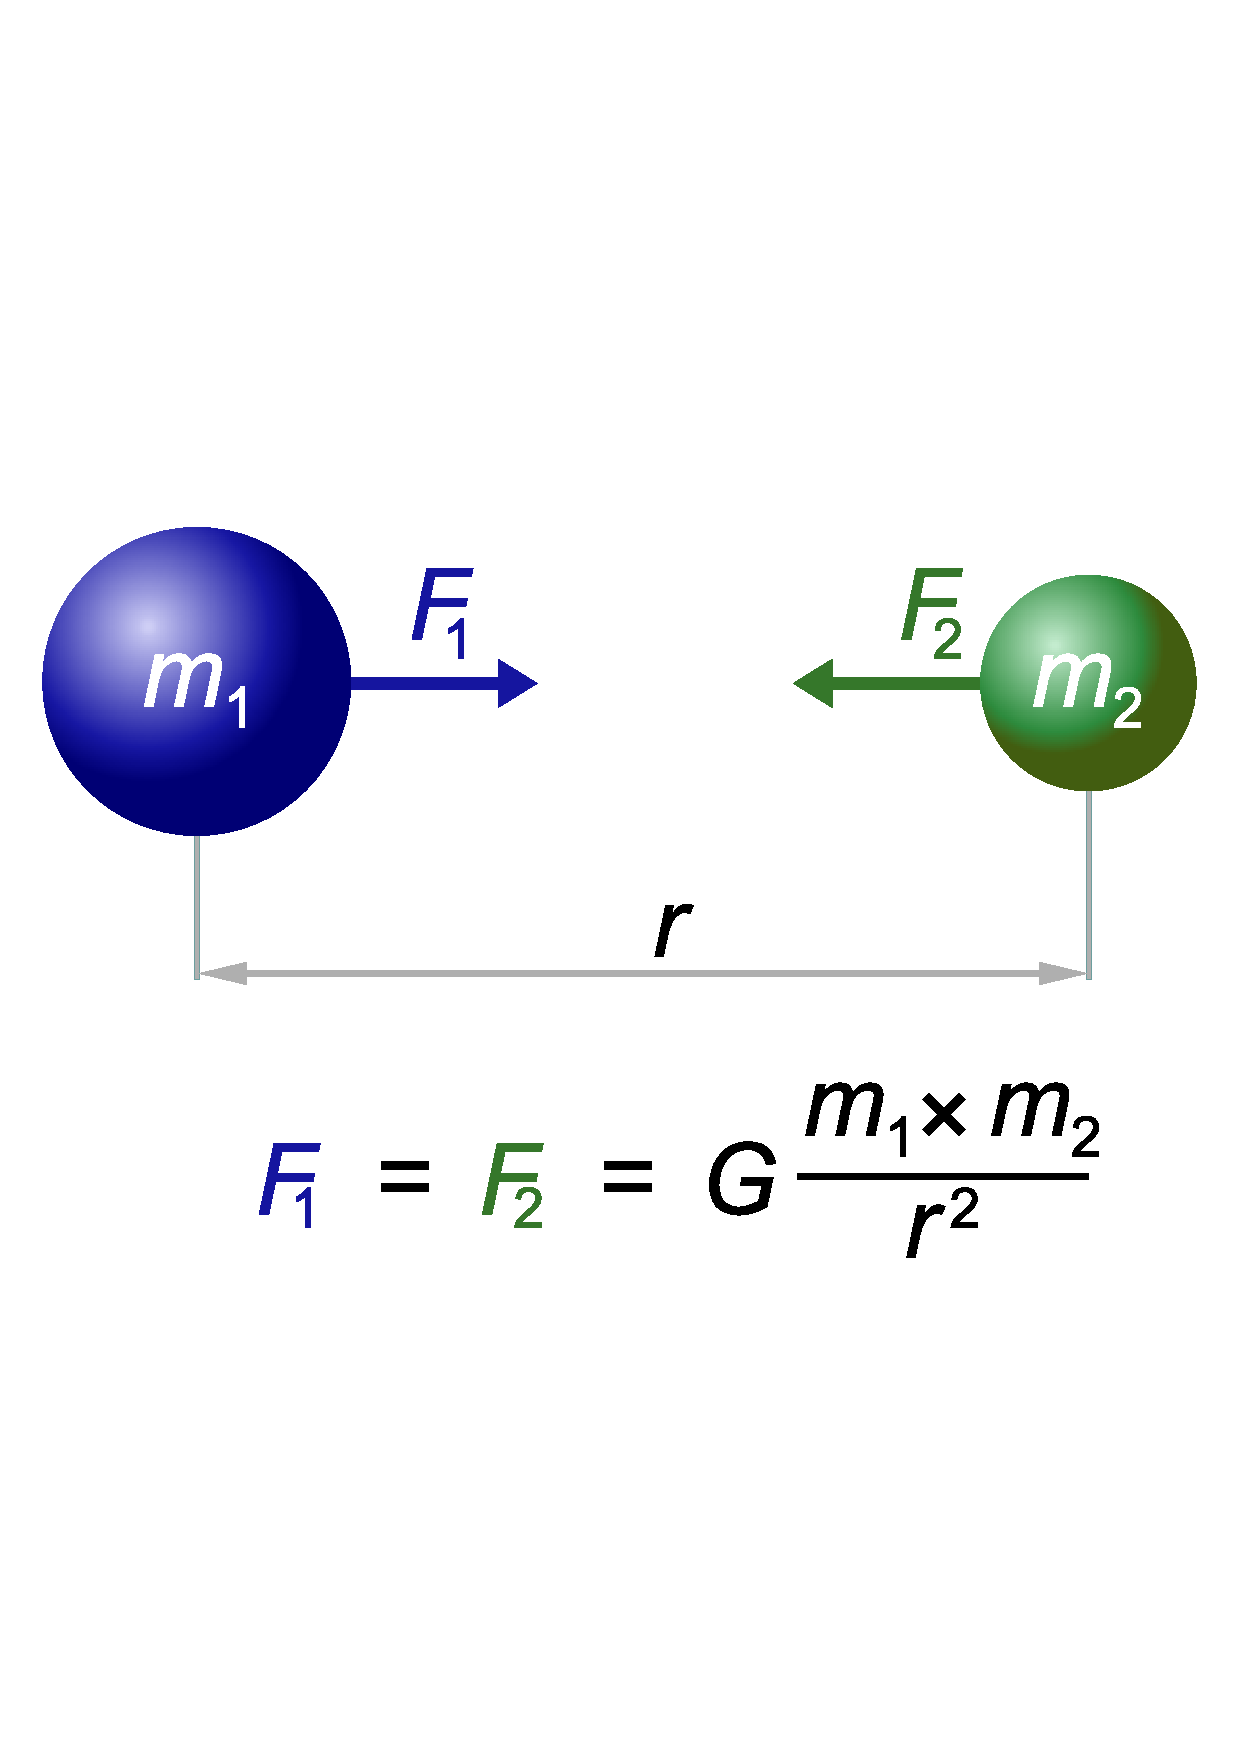
\includegraphics[width=0.35\textwidth]{./figures/universalGravitation.pdf}
\caption{\label{universalGravitation}万有引力定律:$F = Gm_1m_2/r^2$
}
\end{figure}

根据当时已经有了地球半径, 日地距离等精确的测量数据. 牛顿利用微积分证明地球的引力是使月亮围绕地球运动的向心力, 同时也证明了在太阳引力作用下, 行星运动符合开普勒运动三定律.
在哈雷的敦促和资助下, 1686年底, 牛顿完成了伟大著作$\ll$自然哲学的数学原理$\gg$一书并于1687年出版.

从牛顿发现万有引力定律的过程中, 可以看出, 胡克等人与引力定律的发现擦肩而过. 牛顿高明的地方在于他懂微积分, 并利用微积分解决了胡克等人无解决的数学论证问题.
牛顿的例子告诉我们科学研究不只是要站在巨人的肩上, 还告诉我们\textbf{先进的数学方法在理论证明过程中是至关重要的}.

\subsection{麦克斯韦与麦克斯韦方程组}
麦克斯韦的主要贡献是建立了麦克斯韦方程组, 创立了经典电动力学, 并且预言了电磁波的存在,
提出了光的电磁说. 麦克斯韦是电磁学理论的集大成者.
物理学历史上认为牛顿的经典力学打开了机械时代的大门, 而麦克斯韦电磁学理论则为电气时代奠定了基石.
麦克斯韦之所以能够建立电磁学理论, 是因为不同于法拉第, 麦克斯韦有着极高的数学造诣.
\begin{window}[0,0,{\mbox{%
\fbox{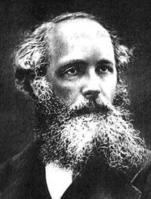
\includegraphics[width=\picwidth,totalheight=\pichigh]{./figures/maxwell.jpg}}}},{}]
麦克斯韦1831年6月13日生于英国爱丁堡. 1847年进入爱丁堡大学学习数学和物理. 1850年转入剑桥大学三一学院数学系学习, 1854年毕业留校任职两年. 1856年在苏格兰阿伯丁的马里沙耳任自然哲学教授. 1860年到伦敦国王学院任自然哲学和天文学教授. 1861年选为伦敦皇家学会会员.
1856-1865年间发表了$\ll$论法拉第的力线$\gg$, $\ll$论物理的力线$\gg$及$\ll$电磁场的动力学理论$\gg$.
1865年春辞去教职回到家乡系统地总结他的关于电磁学的研究成果, 完成了电磁场理论的经典巨著$\ll$电磁理论$\gg$, 并于1873年出版, 1871年受聘为剑桥大学新设立的卡文迪什试验物理学教授, 负责筹建著名的卡文迪什实验室, 1874年建成后担任该实验室主任, 1879年11月5日在剑桥逝世.
\end{window}

麦克斯韦出生的那年(1831), 40岁的法拉第就发现了电磁感应: 一块磁铁穿过一个闭合线路时, 线路内就会有电流产生.
比法拉第小40岁的麦克斯韦大约于1855年才始研究电磁学, 在研究了法拉第关于电磁学方面的理论后, 坚信法拉第的新理论包含着真理. 于是他抱着给法拉第的理论``提供数学方法基础''的愿望, 决心把法拉第的天才思想以清晰准确的数学形式表示出来.

麦克斯韦的第一篇电磁方面的论文$\ll$论法拉第的力线$\gg$受到了法拉第的称赞和鼓励:``这是一篇出色的论文, 但是,你不应该停留在用数学来解释我的观点,你应该突破它!''
在该篇论文中, 麦克斯韦將法拉第想出的力线延伸为装满了不可压缩流体的力管, 利用数学的类比方法, 并借用流体力学的一些数学框架,推导出一系列电磁学理论初形.
而后麦克斯韦的工作不再是法拉第观点纯粹的数学翻译, 而是作了重大的引申和发展.

在第二篇论文
$\ll$论物理学的力线$\gg$, 提出了``分子渦流模型'' , 认为磁场是一种旋转现象, 合理地解释了各种磁场现象及其伴隨的作用力, 并能够推导出安培定律, 法拉第感应定律等等.
在此基础上, 引进了``位移电流''这个具有决定性意义的概念. 并通过严密的数学推导, 求出了位移电流的方程式.根据这个科学假设, 麦克斯韦推导出两个高度抽象的微分方程式(1865年最终完善), 这就是著名的麦克斯韦方程式.

1864年麦克斯韦发表了他的第三篇电磁学方面的论文$\ll$电磁场动力学$\gg$. 该篇论文中有一节标题为电磁场一般方程式. 麦克斯韦提出了由20个等式和20个变量组成的方程组. 后经奥利弗$\cdot$黑维塞和约西亚$\cdot$吉布斯以向量分析的形式重新表达得到现在通用的形式. 具体微观的微分和积分形式如下:
\begin{eqnarray}
\nabla\cdot \mathbf{E} = \frac{\rho}{\varepsilon_0} & & \int\!\!\!\!\int_{\mathbb{S}}\!\!\!\!\!\!\!\!\!\!\!\!\!\!\;\;\;\bigcirc\,\,\mathbf E\cdot\mathrm{d}\mathbf{s} = \frac{Q}{\varepsilon_0}\nonumber\\
\nabla \cdot \mathbf{B} = 0
& &\int\!\!\!\!\int_{\mathbb{S}}\!\!\!\!\!\!\!\!\!\!\!\!\!\!\;\;\;\bigcirc\,\,\mathbf B\cdot\mathrm{d}\mathbf{s} = 0\nonumber\\
\nabla \times \mathbf{E} = - \frac{\partial \mathbf{B}} {\partial t}
& & \oint_{\mathbb{L}} \mathbf{E} \cdot \mathrm{d}\boldsymbol{\ell}= - \frac {\mathrm{d} \Phi_\mathbf{B}}{\mathrm{d} t}\nonumber\\
\nabla \times \mathbf{B} = \mu_0\mathbf{J} + \mu_0 \varepsilon_0 \frac{\partial \mathbf{E}} {\partial t} & &\oint_{\mathbb{L}}\ \mathbf{B} \cdot \mathrm{d}\boldsymbol{\ell}= \mu_0 I + \mu_0 \varepsilon_0 \frac {\mathrm{d} \Phi_\mathbf{E}}{\mathrm{d} t}\nonumber
\end{eqnarray}

麦克斯韦还于1873年出版了他的$\ll$电磁通论$\gg$.
这是一部电磁理论的经典著作, 系统地总结了19世纪中叶前后, 库仑, 安培, 奥斯特, 法拉第和他本人对电磁现象的研究成果, 建立了完整的电磁理论.

从麦克斯韦总结出电磁学的麦克斯韦方程组的过程中, 我们不难发现, 数学使得麦克斯韦在电磁学的研究中占了绝对优势. 尽管强于实验的法拉第研究电磁比麦克斯韦早得多,并有很多新奇的思想及开创性的成果, 但却无法用数学这一强大的工具表达出来. 也因此而使他的研究成果受到了进一步发展的限制. 而麦克斯韦应用数学符号成功的刻画出了法拉第的研究成果, 使电磁理论有了跨越式的发展.
麦克斯韦的实例不仅告诉我们实验固然重要, 同时还告诉我们, \textbf{能否用简捷的数学语言将实验及理论表达出来, 并推导延伸为更深课的理论和结论是至关重要的}.


\subsection{孟德尔与遗传规律}
生物学中一个重要的发现, 就是遗传规律. 1900年孟德尔遗传规律的重新提出, 标志着生物学进入到了实验生物学阶段, 对于整个生物学, 遗传规律的发现显然是举足轻重的. 而孟德尔之所以能发现别人没能发的这一规律, 主要依赖于其将数学引入了生物学研究. 下面介绍一下孟德尔的生平以及发现遗传规律的过程.

\begin{window}[0,0,{\mbox{%
\fbox{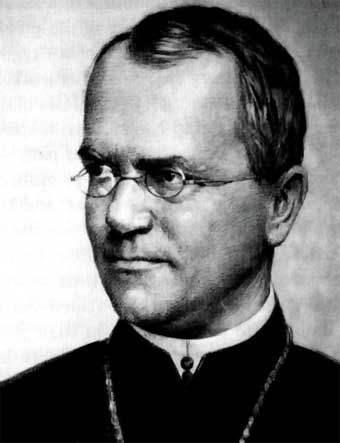
\includegraphics[width=\picwidth,totalheight=\pichigh]{./figures/mendel.jpg}}}},{}]
1822年7月20日孟德尔生于奥地利的海因岑多夫(今捷克的海恩塞斯). 先后进入特罗保的预科学校, 奥尔米茨哲学院学习. 后因家贫而于1843年辍学做了修士. 1851年-1853年在维也纳大学学习物理, 化学, 数学, 动物学和植物学. 从维也纳大学毕业后重回修道院. 1854年被委派到布吕恩技术学校任物理学和植物学的代理教师, 在那里工作了14年, 其间进行了豌豆杂交的实验. 1884年1月6日卒于布吕恩.

孟德尔的豌豆杂交实验:将高杆和矮杆豌豆进行了人工杂交, 获得了只产生高植株的种子. 这种种子自花受精时, 产生的高植株和矮植株是3:1. 这样产生的矮植株总是繁育同样的后代, 但是三个高植株中只有一个如此,另两个仍是以三与一的比例生出高和矮的植株来.
\end{window}

孟德尔认为每一植株都具有两个决定高度性状的因子, 每一亲体赋予一个因子. 高的因子(D)是显性, 而矮的因子(d)是隐性, 因此杂交后第一代的植株全都是高的(Dd). 当这一代自花受精后, 这些因子在子代中排列可以是两个高因子在一起(DD), 或者两个矮因子在一起(dd), 或者一高一矮(Dd), 一矮一高(dD). 其基本原理如图\ref{meEx}.
\begin{figure}[!htb]
\centering
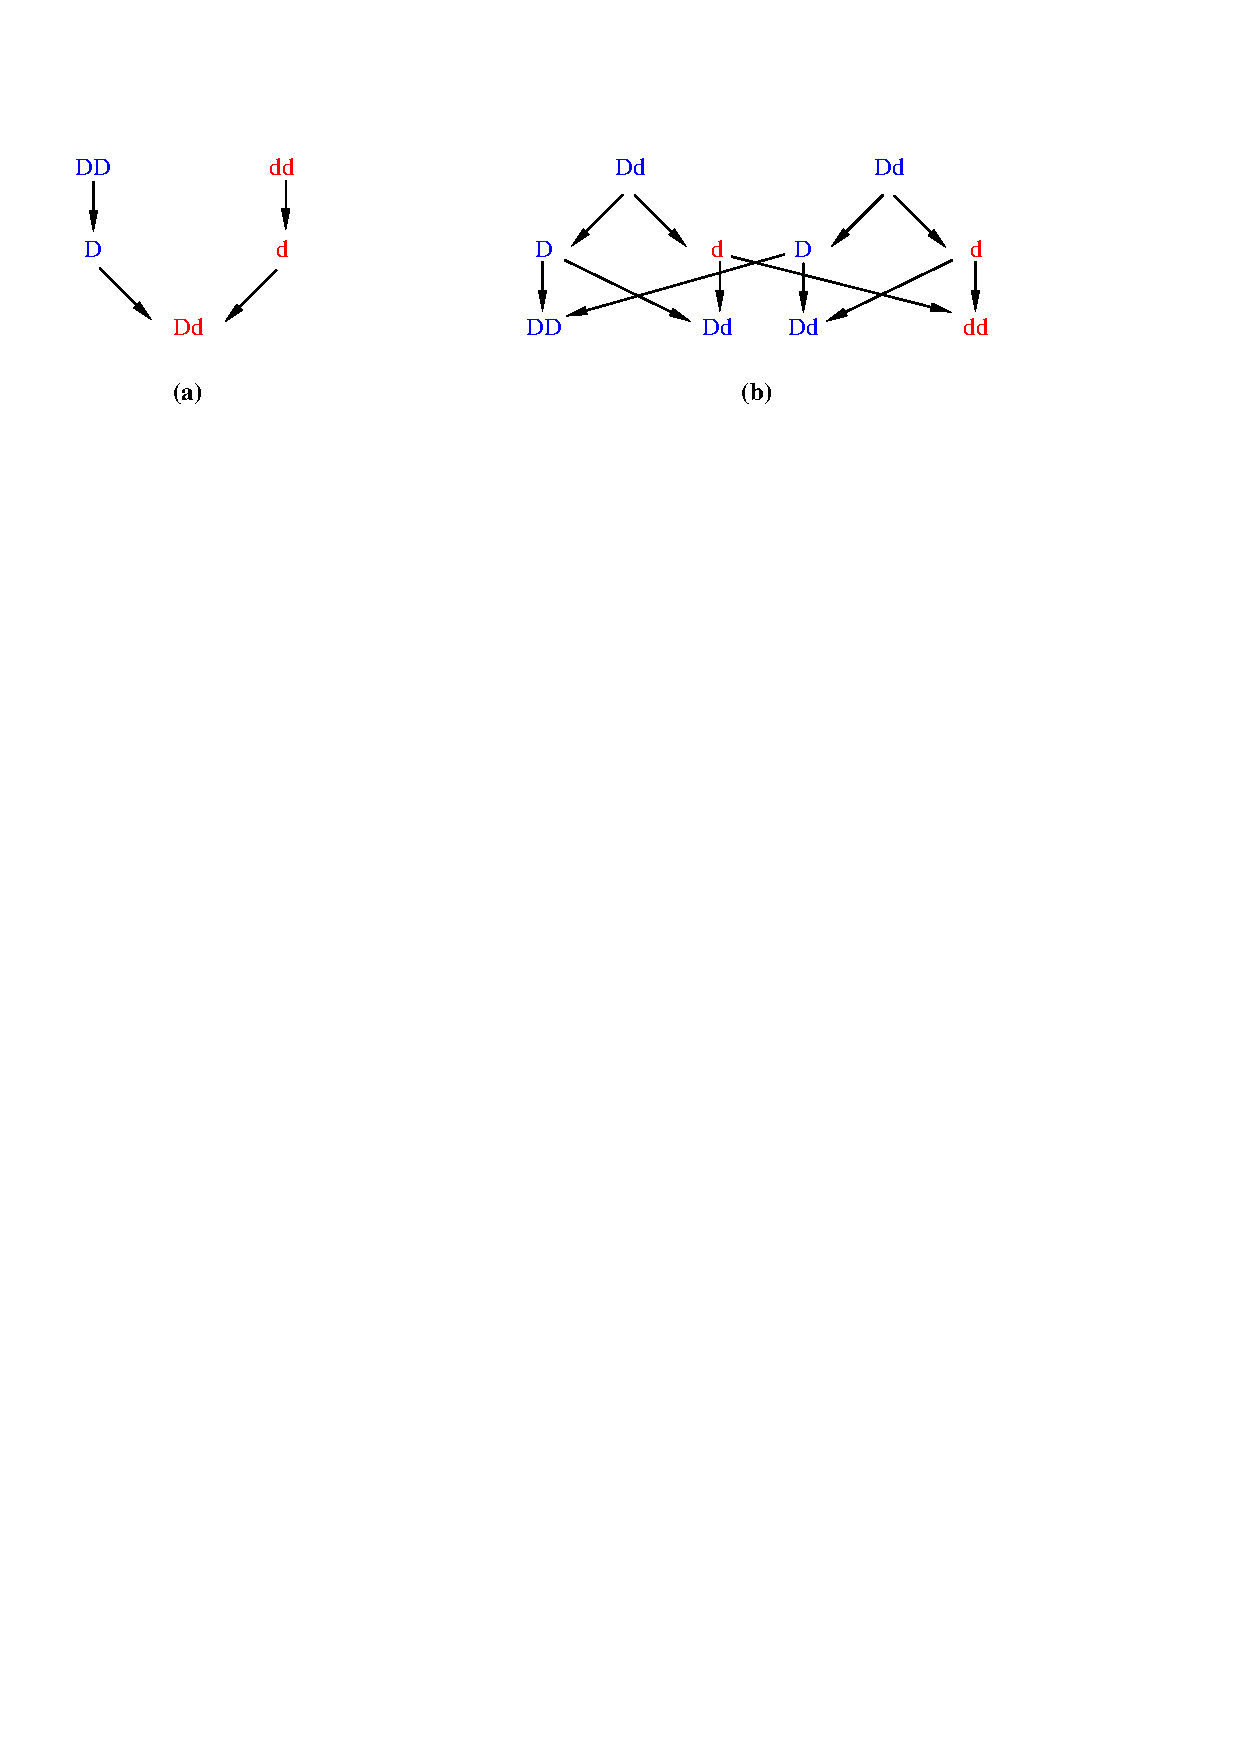
\includegraphics[width = 0.7\textwidth]{./figures/meEx.pdf}
\caption{\label{meEx}孟德尔豌豆杂交实验原理}
\end{figure}
孟德尔于1865年在布吕恩自然科学研究协会上报告了他的研究结果. 1866年又在该会会刊上发表了题为$\ll$植物杂交试验$\gg$ 的论文. 他在这篇论文中提出了遗传因子(现称基因)及显性性状, 隐性性状等重要概念, 并阐明其遗传规律, 后人称之为孟德尔定律(包括基因的分离定律及基因的自由组合定律). 但是他的这些发现当时并未受到学术界的重视. 直到1900年, 孟德尔定律才由3位植物学家荷兰的德弗里斯, 德国的科伦斯和奥地利的切尔马克通过各自的工作分别予以证实, 成为近代遗传学的基础. 从此孟德尔也被公认为科学遗传学的奠基人.

从孟德尔发现遗传规律的过程中, 我们不难发现孟德尔在大学学习的数学知识
为其发现规律奠定了基础. 在实验结果的分析阶段, 他运用数学统计学的方法对实验结果进行了分析, 对实验数据进行了合理的处理. 大胆的假设并从中归纳出了一般规律. 将数学研究手段引入到生物学研究也是当时孟德尔区别于其他生物学研究者最明显的地方, 这也是为什么只有孟德尔发现了遗传规律的原因.
孟德尔的例子告诉我们的除了做科学研究要耐得住寂寞外, 还告诉我们\textbf{数学在实验结果的分析过程中是至关重要的}.

\section{总结}
科学史告诉我们, 数学在理论分析, 结果表示, 实验数据处理等种个科学进步的过程中都有很重要的作用, 这看起来似乎这么肤浅的道理, 却是一个个科学史上的天才的鲜活演绎. 作为科学院的研究生, 所有人都深知这个道理,  将来(如果)从事科学研究, 数学是必不可少的工具(当然这里的工具还可以推广到计算机, 不过这是题外话). 但科学史还告诉我们更深刻的道理:
\begin{itemize}
\item \textbf{现有的科学成就都是成于数学!}
因为数学, 开普勒发现了开普勒定律, 而更有机会发现该定律的第谷没能发现; 因为数学, 牛顿发现了万有引力定律, 而更有机会发现该定律的胡克等人没能发现; 因为数学, 麦克斯韦总结出了麦克斯韦方程组, 而更有机会发现该方程组的法拉第没能发现;
因为数学, 孟德尔发现了遗传规律, 而更有机会发现该定律的专业生物研究者没能发现; 因为数学, ... 发现了...这样的例子还很多, 甚至可能说无一例外! 牛顿力学, 相对论, 量子力学...哪一个学科又不是成于数学呢?
\item \textbf{自然科学的进步依赖于数学的进步}. 伟大的牛顿力学(特别是万有引力定律)依赖于微积分发现, 或者微积分的发现促成了伟大的牛顿力学(特别是万有引力定律)的产生与发展.
因此, 当我们走到无法前进的地步时(就像当时胡克等人卡在了万有引力产生之前一样),
我们是不是该停下脚步, 想想我们在数学上有没有新的发展, 新的进步, 新的突破.
\end{itemize}
科学世界用一部辉煌的科学史正在, 也将继续不断的告诉人们: 谁能撑握数学, 谁就能拥有打开科学大门的钥匙.

\textbf{在日益发展的今天, 数学也并非只作用于科学, 它存在生活的方方面面!} 虽然作为科学院的研究生, 很大一部分人毕业后并不从事科研, 但数学仍然是工作中提高效益的法宝. 比如, 搞经济的用数学模型研究宏微观经济, 搞市场调研的用数学统计学进行市场调查及预测, 搞分险评估的用数学概率理论进行风险分析以指导金融投资, 搞股票的用数学预测方法预测股市的走向, 搞企业管理的用数学规划和运筹学等数学优化方法提高企业的...

因此, 撑握数学这一强大工具的人, 才能撑握世界(当然这里的工具还可以推广到计算机, 不过这是题外话). 因此, 作为明日世界主人的我们, 必需学好数学, 用好数学!



\begin{thebibliography}{99}
\bibitem{0} The Story of Science. BBC. \textit{http://topdocumentaryfilms.com/story-of-science/}
\bibitem{1} Johannes Kepler. \textit{http://en.wikipedia.org/wiki/Johannes\_Kepler}
\bibitem{2} Kepler's laws of planetary motion. \\ \textit{http://en.wikipedia.org/wiki/Kepler\%27s\_laws\_of\_planetary\_motion}
\bibitem{1} Isaac Newton. \textit{http://en.wikipedia.org/wiki/Isaac\_Newton}.
\bibitem{}Newton's law of universal gravitation. \textit{http://en.wikipedia.org/wiki/Law\_of\_universal\_gravitation}
\bibitem{2} James Clerk Maxwell. \textit{http://en.wikipedia.org/wiki/James\_Clerk\_Maxwell}.
\bibitem{3} Maxwell's equations
    \textit{http://en.wikipedia.org/wiki/Maxwell\%27s\_equations}
\bibitem{4} Gregor Johann Mendel. \textit{http://en.wikipedia.org/wiki/Gregor\_Mendel}
\bibitem{5} Mendelian inheritance.
    \textit{http://en.wikipedia.org/wiki/Mendelian\_inheritance}
\end{thebibliography}

%\newpage
%\problemlist{给刘红老师的一封信}
%\noindent 刘红老师:
%
%您好! 首先感谢您给我们带来精彩的近现代科学技术史, 并且强调了一些很有意义以及我们今后科研需要注意的问题. 近现代科学技术史是一门很有意义, 也很有意思的课程, 它就像是一本科学人物传记, 但又不同于人物传记. 虽然选您课的同学并没有我想象的多, 但您仍然充满激情的讲课方式使得效果很好. 当然您的课程还可以讲得更好, 为此我提一些我个人对本课程的看法, 当然我说的也不一定对, 仅供您参考:
%\begin{itemize}
%\item \textbf{强调实验, 对于理论, 应说明哪些是假设, 哪些是假说.}
%
%科学史中的日心说替代了地心说, 给了我们深刻的启示, 不要迷信权威以及现有的主流知识. 地心说盛行了千年, 最终也被证明是错的. 相对论, 量子力学等等也才百年而矣. 以德布罗意波为例, 从德布罗意的厚厚的博士论文中, 不难发现其推导如下:\\
%\begin{problem}
%由假说$E=h\nu$得
%\[
%E=h\nu=h\frac{1}{\tau^*}=h\frac{v}{v\tau^*}=h\frac{v}{\lambda} \ \
%\footnote{偷换概念:$v\tau^*=\lambda$ ,其中$v$是粒子运动速度}
%\]
%又由爱因斯坦质能方程(亦属假说):$E=mc^2$将光速$c$偷换为$v$
%得
%\[
%E=mv^2
%\]
%由以上两式联立可得
%\[
%\lambda=\frac{h}{mv}
%\]
%\end{problem}\\
%推导的前提依据都是假说, 并且推导本身就有问题. 再如证明爱因斯坦相对论的实验也是有问题的, \textcolor{blue}{光经过太阳周围发现了偏转是不是能证明引力场弯曲了还有待考就: 太阳是个气球, 表面的气体是不均匀的, 光线经过太阳表面必然发生折射.} 但在讲这个实例时, 好像都没有涉及折射的可能.
%
%对于哪些是建立在假说基上的问题, 我觉得科学史的课程也应该给于说明, 否则让人觉得这些已经是不争的事实了, 这样是不是可能造成一些误导, 使得一些``哥白尼''没有产生. 而实验的事实是不争的, 是什么现象就是什么现象, 对于实验的解释倒可以有多种.
%\item \textbf{作业次数不限于一次, 形式不限于报告.}
%个人觉得该课程的作业可以有更多的形式及更多次. 比如课程中可以插入四次不同形式的作业: 作业可以是小组形式的讨论, 结果可以是每个小组一名同学上台讲(可以有课件); 也可以是对某些科学家的理解(上百字的简短评论); 当然也可以是现在的这种形式, 一篇报告.
%\item \textbf{穿插更多名人的趣闻, 最好能反应人物特征.}
%从我听课过程中,  我感觉得到在认真听的同学并不多. 我觉得教师可以不用完成教学大纲的内容, 但必需要吸引学生. 教师讲了100个知识(讲的枯燥), 但学生只听10个, 不如教师讲30个知识(讲的精彩), 学生学30个知识. 因此, 可以在课堂上引入更多的趣闻, 故事式的上课方式未必不好.
%\end{itemize}
%
%希望我的看法能够对该课程有所帮助, 另外我在看BBC拍的记录片$<<$科学的故事(The Story of Science)$>>$, 讲的很不错, 我觉得老师你可以借鉴一下.
%
%\vspace{1cm}
%
%\rightline{周吕文}
%\rightline{2011.11.12}

\end{document} 
